\documentclass[11pt,includemp,a4paper]{article}
%\documentclass[11pt]{book}
%\usepackage{pspicture}
%\usepackage{pstricks}
\usepackage{hyperref}
\usepackage{fancyhdr}
%\usepackage{pict2e}
\usepackage{graphicx}
\usepackage{amsmath}
\usepackage{amssymb}
%\usepackage[UTF8]{ctex}
\usepackage{fontspec}
\usepackage{color}
%usepackage{amsmath}
\usepackage[BoldFont,SlantFont,CJKchecksingle]{xeCJK}

\pagestyle{fancy} \markboth{}{}


\setlength{\parindent}{12pt} \setlength{\parskip}{3pt plus1pt
minus2pt} \setlength{\baselineskip}{20pt plus2pt minus1pt}
\setlength{\textheight}{21true cm}
\setlength{\textwidth}{14.5truecm} \setlength{\topmargin}{1cm}
\setlength{\oddsidemargin}{1cm} \setlength{\parindent}{.75cm}
\setlength{\unitlength}{1cm}


\title{21CMA相关机操作手册}
\author{顾俊骅、李宽君}


\begin{document}
\maketitle
\section{相关机外部接口}
相关机的正面、背面和位于背面下方的接口分别如图\ref{fig:daq_front}、\ref{fig:daq_back}、\ref{fig:daq_port}所示。
\subsection{开机前检查}
务必确保\textit{进风口}和\textit{出风口}前没有任何遮挡物,否则将影响散热。\\
\subsection{相关机通电和连接}
电源:标准220V接地插座\\
射频线:使用SMA接口,与外部输入的射频信号连接\\
光纤:相关机的输出,使用一对光纤,与采集计算机相连\\
\subsection{其他连接}
可外接一个VGA显示器、一套USB鼠标键盘。除非进行错误排查,否则不应当进行任何操作。\\

\subsection{相关机的\textcolor{red}{电源按钮-相关机日常采集过程中唯一需要进行操作的按钮}}
按一下即接通内部电源\\
再按一下则断开内部电源。\\
\begin{figure}
    \begin{center}
        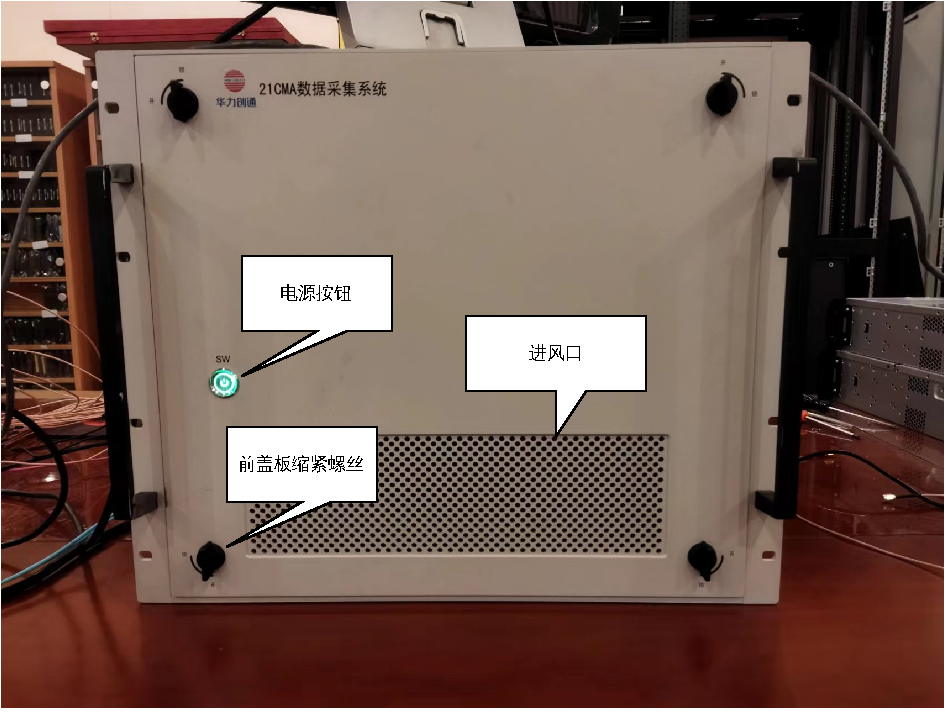
\includegraphics[width=0.5\textwidth]{front.pdf}
    \end{center}
    \caption{\label{fig:daq_front}相关机正面}
\end{figure}

\begin{figure}
    \begin{center}
        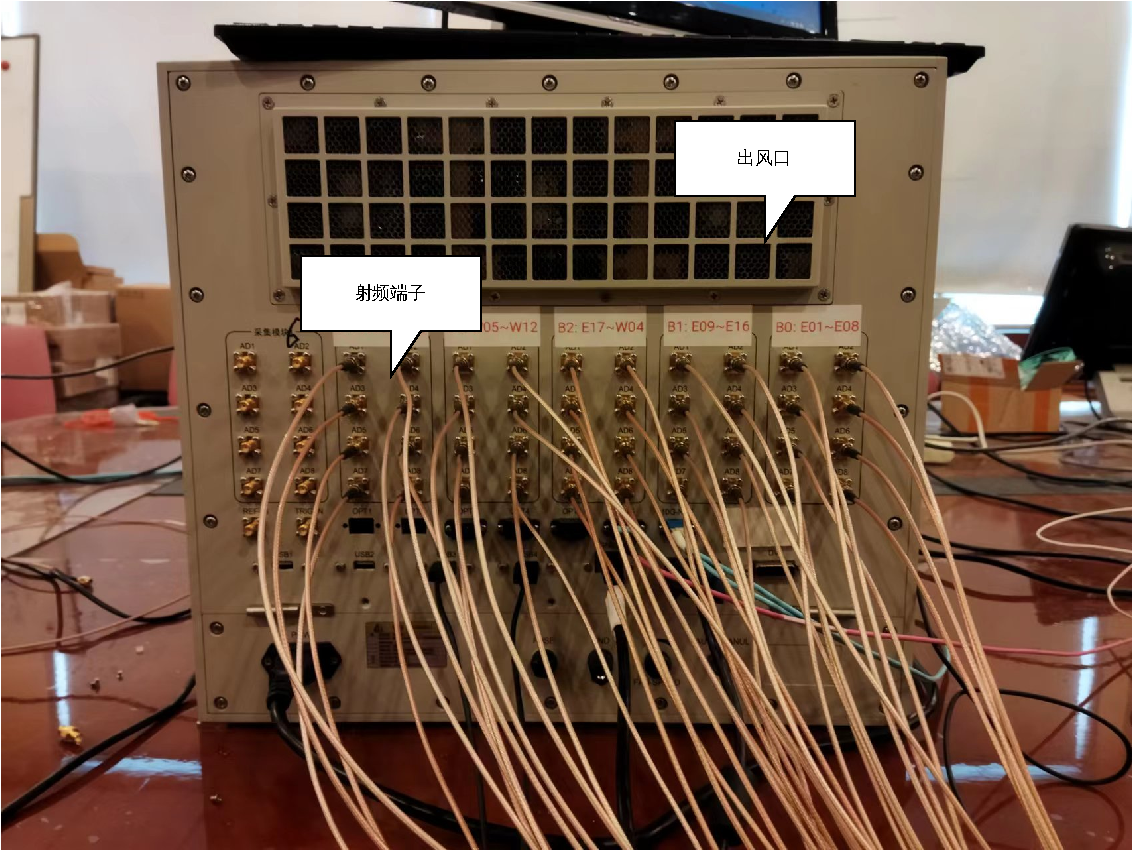
\includegraphics[width=0.5\textwidth]{back.pdf}
    \end{center}
    \caption{\label{fig:daq_back}相关机背面}
\end{figure}


\begin{figure}
    \begin{center}
        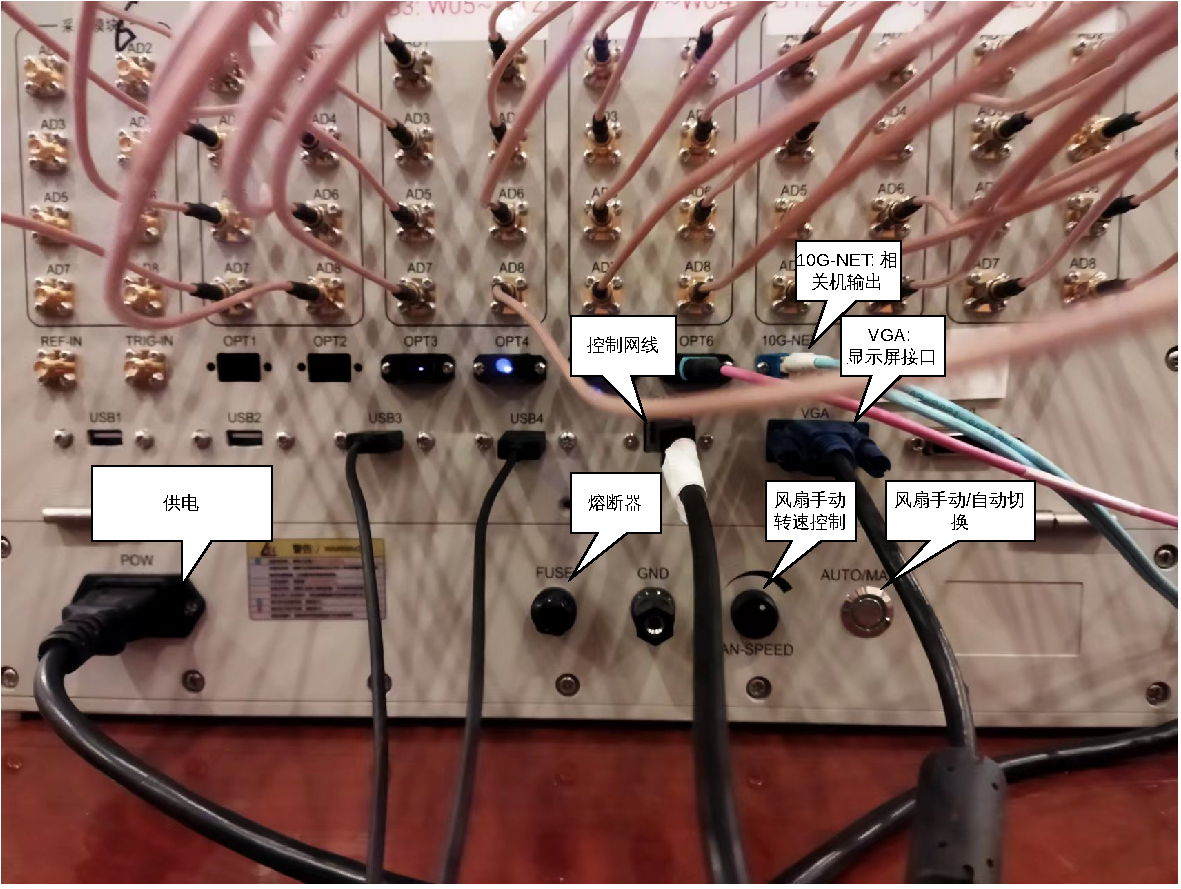
\includegraphics[width=0.5\textwidth]{port.pdf}
    \end{center}
    \caption{\label{fig:daq_port}相关机接口}
\end{figure}


\section{启动、停机、采集操作}
采集系统正常运行时,必然处于“断电”、“关机”、“准备完毕”、“正在采集”这四个状态之一。本节将阐述如何使系统在这些状态之间进行切换。状态转移方式如图\ref{fig:states}所述。
\begin{figure}
    \begin{center}
        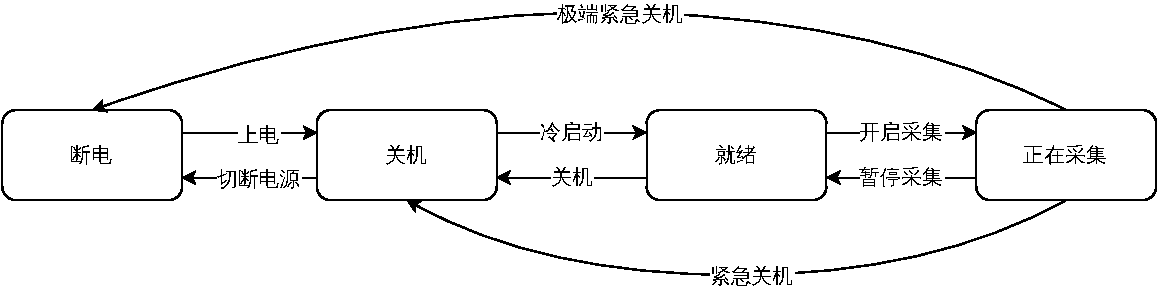
\includegraphics[width=0.75\textwidth]{state_diag.pdf}
    \end{center}
    \caption{\label{fig:states}系统状态转移图}
\end{figure}
\subsection{上电}
本操作假定系统处于完全切断电源的“断电”状态。
\label{ssec:prepare}
\begin{enumerate}
    \item 将全新的硬盘插入采集计算机盘位,八个盘位插满
    \item 采集计算机通电
    \item 相关机通电
\end{enumerate}
完成本操作后,系统将进入“关机”状态。

\subsection{冷启动}
\label{ssec:cold_start}
冷启动是指从“关机”状态开始,使系统进入“就绪”状态,等待执行进入采集的命令,执行本操作的前提是完成\ref{ssec:prepare}或者\ref{ssec:shutdown}中所述操作,并处于“关机”状态。

操作流程如下
\begin{enumerate}
    \item 按相关机电源按钮,开机
    \item 采集计算机开机,待进入登录界面
    \item 用户名******, 密码******(具体内容口述传达)
\end{enumerate}
完成本操作后系统将进入“就绪”状态。

\subsection{开启采集}
\label{ssec:daq}
本操作将是系统进入“正在采集”状态。执行本操作的前提是经由\ref{ssec:cold_start}操作,或者经由\ref{ssec:stop}操作进入“就绪”状态。
\begin{enumerate}
    \item 执行命令 cd $\sim$/src/newdaq
    \item 执行命令 ./run.sh
\end{enumerate}
完成本操作后,系统将处于“正在采集”状态。

\subsection{暂停采集}
\label{ssec:stop}
暂停采集是指是系统从“正在采集”状态中退出,转而进入“就绪”状态。执行本操作的前提是系统经由此前\ref{ssec:daq}所述操作,并正处于“正在采集”状态之中。

操作流程如下
\begin{enumerate}
    \item 执行命令 cd $\sim$/src/newdaq
    \item 执行命令 ./stop.sh
\end{enumerate}
完成本操作后,系统将进入“就绪”状态。

\subsection{关机}
\label{ssec:shutdown}
本操作的目的是使系统进入“关机”状态。并为完全断电做准备。执行本操作的前提是系统经由\ref{ssec:cold_start}或者\ref{ssec:stop}所述操作,进入“准备完成”状态。

操作流程如下
\begin{enumerate}
    \item 执行命令 cd $\sim$/src/newdaq
    \item 执行命令\footnote{关机操作如此设计的出发点,是防止误操作,特别是在远程操作的过程中防止意外关机} bash shutdown.sh a2b1c4d5(关闭采集系统)
    \item 执行命令 sudo poweroff(关闭采集计算机)
    \item 按相关机的电源按钮,切断相关机内部供电,相关机内部风扇完全停止转动(切断电源)
\end{enumerate}
完成本操作后,采集系统将进入“关机”状态。

\subsection{切断电源}
\label{ssec:cut_power}
本操作的目的是使系统进入完全断电状态,执行本操作的前提是系统经由\ref{ssec:prepare}或者\ref{ssec:shutdown}所述操作,进入“关机”状态。
操作流程如下
\begin{enumerate}
    \item 通过关闭空气开关等方法,切断系统供电
    \item 拔出所有硬盘
\end{enumerate}
执行完本操作后,系统将处于“断电”状态。

\subsection{紧急关机}
在某些情况下(例如即将停电,且UPS余电不足以支持正常关机),需要在极短时间内完成关机,不论系统处于任何状态,都可以执行如下操作完成:
\begin{enumerate}
    \item 执行命令 cd $\sim$/src/newdaq
    \item 执行命令 bash shutdown.sh a2b1c4d5 (关闭采集程序)
    \item 执行命令 sudo poweroff(关闭采集计算机)
    \item 按相关机的电源按钮,切断相关机内部供电,相关机内部风扇完全停止转动(切断电源)
\end{enumerate}

完成本操作后,系统将处于“关机”状态。紧急关机和一般关机的区别在于是否在之前的步骤中执行了暂停采集操作。

\subsection{极端紧急关机}
在某些极端情况(例如设备起火),需要立刻切断电源,操作方法是尽一切可能,完全立刻切断系统供电,并进行灾后处置。

\section{采集过程中的例行维护}
\subsection{系统状态监控}
假设采集计算机的ip地址是192.168.4.100,并且假设系统处于“正在采集”,则可以通过访问\url{http://192.168.4.100:8000}访问采集计算机的监控页面,从中可以读取板卡温度、板卡状态和实时频谱。\\
如果出现板卡温度过高,板卡状态错误,实时频谱异常,应尽快记录并微信或者电话告知。

\subsection{日常巡检}
每日巡检至少3次,之间间隔4小时,观察系统外观是否正常,确保空调正常运行,白天工作时间应当经常访问监控页面,了解系统工作状态。

\subsection{换盘}
\begin{enumerate}
    \item 采集系统每天写入数据量约为1.5 TB,故若采用2TB硬盘,每天写满一块盘,若采用4TB硬盘,则每两天写满一块盘
    \item 每天应当检查是否有硬盘写满,若写满,则当天应当更换该硬盘。换下的硬盘应当贴上标签,并写明前一日的日期
    \item 每天检查采集计算机的磁盘盘位,若红色LED闪烁,则表明该盘位中的硬盘已经写满
    \item 直接将写满的硬盘退出,并插入一块全新的硬盘。插入后采集系统将自动识别,并进行格式化,不需要手动操作。
\end{enumerate}




\end{document}
